\section{Analytical Model for Query Response Time}
\label{sec:model}
In this section we present an analytical model for an upper bound on the query response time and parametrically study its dependence on the Internet topology and replication factor $K$. While the simulation framework of Section \ref{sec:evaluation} shows the response time performance of DMap based on the current Internet topology, this analytical model allows us to estimate its performance based on a predicted future Internet model.
\subsection{The Jellyfish Model}
An accurate parametric model of the Internet topology is known to be a difficult endeavor due to the inherent complexities in routing policies, detour paths and limited visibility of the intra-AS structure~\cite{HeSF09}. The Jellyfish model, however, has been found to closely follow the evolution of the Internet topology at a relatively coarse scale~\cite{tauro-jellyfish}. In this paper, we build a Jellyfish model based on the PoP-level Internet topology. We first label the node with the highest degree as the root $v_0$ and the maximal clique\footnote[1]{clique: a completely connected subgraph of $G$.} containing $v_0$ as the {\em core}, denoted as $Shell\textrm{-}0$. Let $v$ be a non-root node and $j$ a non-negative integer. The smallest path length\footnote[2]{path length: the number of edges in the path, $i.e.$, that of the involved PoPs in the path minus 1.} from $v$ to a node in the core is its {\em distance to the core}. We use $Shell\textrm{-}j$ to denote the set of nodes whose degree is more than 1 (intermediate nodes) and whose distance to the core is $j$. We use $Hang\textrm{-}j$ to denote the set of nodes whose degree is 1 (leaf nodes) and whose distance to the core is $j+1$. These are standard notations in the Jellyfish model~\cite{HeSF09}. Then we have
\[
Layer(j) = Shell\textrm{-}j \cup Hang\textrm{-}(j-1) \textrm{~~for~}j \ge 1,
\]
and $Layer(0)=Shell \textrm{-} 0$. We further denote the total number of layers in the Internet PoP topology as $N$ and the percentage of nodes in layer $j$ by $r_j$; if $n$ is the total number of nodes in $G$, then $r_j = \left| Layer(j) \right| / n$. The separation of one degree nodes at each layer distinguishes between stub connections and transit connections which makes the model much closer to the Internet topology than a standard tree structure.

\subsection{Upper Bound for Query Response Times}
Following the above model, if we assume no peer links between the nodes inside each layer, then the distance between any two nodes $s$ and $t$ (in layers $j_s$ and $j_t$ respectively), $d(s, t)$,  is at most $j_s + j_t + 1$. Note that since the core forms a completely connected graph, all hops in the core are of length one.  To drive a simple parametric upper bound for the query response time, we assume that the network address space is uniformly distributed among the PoPs and all addresses within a PoP behave in an identical fashion. Following the algorithm described in Section \ref{sec:design}, let the source of a GUID query belong to PoP $s$ and let $t_1, t_2, \ldots, t_K$ be the destination PoPs for the query determined by the $K$ hash functions $h_1, h_2, \ldots, h_K$ applied on the GUID $G$. Assuming a linear relationship between PoP path length and response time, the query response time $\tau(s, G)$, is thus given by

\begin{equation}
\tau(s, G) = c_0 \cdot \min_{1 \le i \le K} d (s, t_i) + c_1,
\label{eq:tau}
\end{equation}
where $c_0$ and $c_1$ are constants. In order to average over all possible source and destination PoPs, we treat $d(s, t_i)$ as a random variable and find its probability distribution based on the $r_j$ values defined in the previous subsection. In the analysis, we use the standard notations $Pr (\cdot )$ and $Pr ( \cdot ~|~ \cdot )$ for the probability and conditional probability of argument events, and $ \mathbb{E}( \cdot )$ for the expected value of a random variable.

Given a uniformly selected source PoP, we have $Pr(s \in Layer(j) )= r_j$. Note that since DMap actually chooses a network address uniformly over all possible addresses, the $j^{th}$ layer could include a different number of addresses than the ratio $r_j$. Our analysis assumes the uniform distribution of addresses among PoPs but the model can be easily extended to non-uniform distributions by considering weights $w_s$ proportional to the number of addresses in PoP $s$. Since accurate estimates of such a distribution is not directly available through any of the Internet measurement frameworks, we assume $w_s = 1$ for all $s$. Based on the same assumptions, we have $Pr ( t_i  \in Layer (j_i) ) = r_{j_i}$ for each $i=1, 2, \ldots , K$ and $j_i=0, 1, 2, 3, 4, \ldots, N-1$. Thus the conditional probability of $d ( s, t_i ) \ge l+1$ given that $s \in Layer(j)$ is at most the percentage of nodes in $Layer(l-j) \cup Layer(l+1 - j ) \cdots \cup Layer(N-1) $. (Since $s$ is in $Layer(j)$, $d ( s, t_i ) = l+1$ when $t_i$ is in $Layer(l-j)$, $d ( s, t_i ) = l+2$ when $t_i$ is in $Layer(l+1-j)$ and so on in the worst case). In other words,
\begin{equation}
\begin{aligned}
& Pr\left(d (s, t_i) > l  ~\big|~ s \in Layer(j) \right)  \le  p_{j,l},
\\ \textrm{where }
& p_{j, l} \stackrel{def}{=} r_{l-j} + r_{l+1 - j} + r_{l+2 - j}\cdots
\\ \Rightarrow & \nonumber
Pr \left(  \min_{1 \le i \le K} d ( s, t_i ) > l  ~\big|~ s \in Layer(j)  \right)  \le  p_{j,l}^K,
\\ \Rightarrow & \nonumber
Pr \left(  \min_{1 \le i \le K} d ( s, t_i ) \le l  ~\big|~ s \in Layer(j)  \right)  >  1 - p_{j,l}^K,
\\ \Rightarrow & \label{CDF}
Pr \left(  \min_{1 \le i \le K} d ( s, t_i ) \le  l  \right)  >
\sum_{j=0}^{N-1} r_j ( 1 - p_{j,l}^K ).
\end{aligned}
\end{equation}

This provides an upper bound for the CDF of average distance from the source to the closest destination. Thus the probability that $\min_{1 \le i \le K} d ( s, t_i ) > l$ is at most $ 1 - q_l$, where we define $q_l$ as:
\[
q_{l} \stackrel{def}{=}\sum_{j=0}^{N-1} r_j \left( 1 - p_{j,l}^K \right),
\]
Finally, noting that the diameter of our PoP graph is $(N-1)+(N-1)+1 = 2N-1$ or less,
\begin{equation}
\begin{aligned}
 & \mathbb{E}\left( \min_{1 \le i \le K} d ( s, t_i ) \right) < \sum_{l=1}^{2N-1} (1-q_l)\\
 & \Rightarrow \mathbb{E} \left(\tau(s,G)\right) < c_0 \left(\sum_{l=1}^{2N-1} (1-q_l)\right) + c_1.
\end{aligned}
\end{equation}

\subsection{Analytical Results}

 We use the formulation derived above to study the response time upper bound in three different scenarios with varying number of replicas $K$. The first scenario reflects the current Internet topology, for which we use measured data from the iPlane project~\cite{madhyastha} for setting the parameters $r_j, j = 1,2,\ldots, N$. The data set shows a graph of 193,376 nodes within 8 layers and more than 60\% of the nodes residing in layers 3 and 4. The next two scenarios model the medium-term and long-term future Internet topologies. In order to come up with models for the future Internet, we leverage the following two distinct trends observed from the widely regarded CAIDA measurement framework~\cite{caida-main}: (i) The number of nodes are growing almost linearly with time, (ii) The topology graph is getting flatter with time, i.e. ASs are obtaining more direct paths to the core. Extrapolating these trends, we model the medium-term (5-10 years) future Internet as having 20\% more nodes than present contained in 6 layers. Similarly, the long-term (25-30 years) future Internet model contains double the number of nodes contained in 4 layers. Figure~\ref{fig:resAnalysis} shows the analytical upper bound of average query response time for the three scenarios using the measured least squared error values for ${c_0,c_1} = {10.6,8.3}$. The plot shows that based on the predicted future Internet topology, response time upper bounds for DMap queries become smaller with the evolution. Also, the analysis clearly indicates that increasing the replica number results in diminishing returns beyond a few replicas. We note that actual values for the query response upper bound will typically be smaller than the ones obtained in this analysis, since we did not consider the presence of peering links between nodes in the same layer.\vspace{-0.15in}
\begin{center}
\begin{figure}[t]
\vspace{-0.2in}
\centering
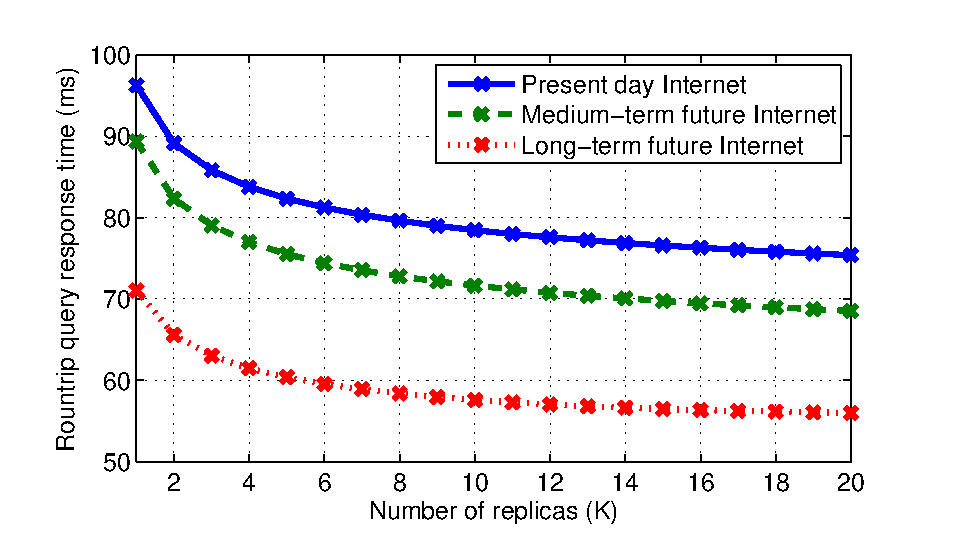
\includegraphics[width=0.5\textwidth]{figures/analysisUpperBound}
\caption{Analytical upper bound of query response times with the Internet topology evolution.}
\label{fig:resAnalysis}
\vspace{-0.2in}
\end{figure}
\end{center} 
%However there might be cases in which multiple tries are required for query resolution, which would increase the total response time from the derived estimates.